%% analyse.tex
%% $Id: analyse.tex 28 2007-01-18 16:31:32Z bless $

\section{Stand der Technik}
\label{ch:Forschungsstand}
Für die Bearbeitung der Forschungsfrage werden verschiedene Technologien bewertet.  Derzeit existiert noch keine bekannte Sprache, die speziell zur Modellierung von Therapien mit Chatbots entwickelt wurden. Aus diesem Grund werden nachfolgend Ansätze betrachtet, die für eine Umsetzung eines \emph{TMA} in Frage kommen. Zunächst werden Plattformen beleuchtet, die eine Erstellung von Chatbots ermöglichen, ohne weitere Programmierkenntnisse zu benötigen. 
%Nachfolgend werden diverse grafische Programmiersprachen betrachtet. Diese bilden Programmstrukturen grafisch ab und werden somit nachvollziehbarer für den Anwender. Eine weitere Kategorie bilden die Auszeichnungssprachen. Diese ermöglichen eine vereinfachte Programmierung zur Strukturierung von Texten. Abschließend werden verschiedene Ansätze im Bereich des Experience Samplings behandelt. Zwar dienen diese zur Erstellung von Studien, allerdings beinhalten sie eine Schnittmenge an Funktionalitäten, die ebenfalls für das Designen von Therapien relevant sind. 

\subsection{Grafische Programmiersprachen}
Diese Art der Programmiersprache bedient sich visueller Elemente um Programmstrukturen verständlich abzubilden. Die visuellen Elemente können auf eine bestimmte Domäne zugeschnitten sein (vgl. \cite{WasistLa94:online}) oder beschränken sich auf die Visualisierung gängiger Programmanweisungen (vgl. \cite{BlocklyG57:online}). In den folgenden Abschnitten werden Chatbot-Plattformen und allgemeine grafische Programmiersprachen betrachtet.


\subsubsection{Chatbot-Plattformen}
%Es gibt eine Vielzahl verschiedener Plattformen zur Entwicklung von Chatbots. Diese sollen insbesondere Personengruppen adressieren, die keine oder nur wenige Programmierkenntnisse besitzen. Die entsprechenden Plattformen verwenden unterschiedliche Ansätze für die Entwicklung. 

Der Konversationsfluss der Chatbots wird auf den Plattformen, wie \emph{Dialogflow} und \emph{IBM Watson} unter anderem als eine Art Baum, ähnlich zur bekannten Ordnerstruktur unter Windows Betriebssystemen, angelegt und dargestellt (vgl. \cite{Dialogfl40:online} \cite{KatalogI56:online}). Chatbot-Plattformen, wie \emph{ManyChat}, \emph{Converse.ai} und \emph{Chatfuel} verwenden Diagramme zur Darstellung eines Chatverlaufes (vgl. \cite{Converse15:online} \cite{WelcomeM66:online}) oder Blocksysteme mit Referenzen auf nachfolgende Blöcke (vgl. \cite{Chatfuel3:online}). Andere Plattformen nutzen keine Darstellung des Verlaufs (vgl. \cite{BotsifyC64:online}). Im Beispiel von \emph{Botsify} oder \emph{Recast.ai} werden nur Verhaltensweisen angelegt, die durch bestimmte Nutzereingaben getriggert werden. 

\begin{figure}[h]
\centering
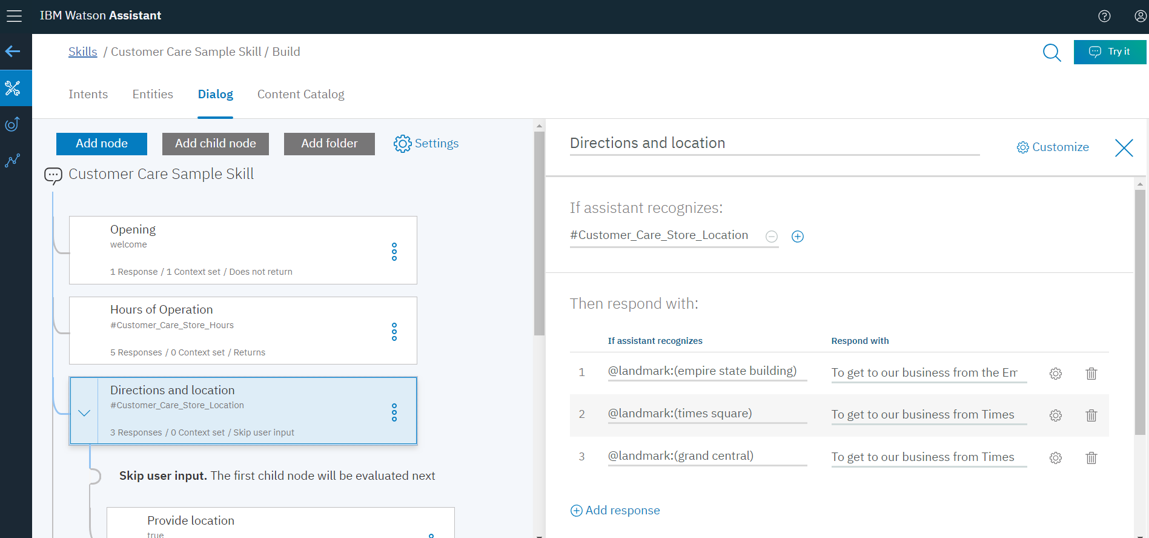
\includegraphics[width=1\textwidth]{pictures/watson}
\caption{Die Chatbot-Plattform \emph{Watson} von \emph{IBM}}
\label{watson}
\end{figure}

Auch in der Handhabung der Nutzereingaben gibt es verschiedene Ansätze. So bieten manche Plattformen die Möglichkeit Antworten für den Nutzer des Chatbots vorzugeben (vgl. \cite{Chatfuel3:online} \cite{WelcomeM66:online}). Andere hingegen verwenden natürliche Sprachverarbeitung um Schlagwörter einzutrainieren. Der Ersteller des Chatbots legt fest, wie der Chatbot auf die entsprechenden Schlagwörter reagiert (vgl. \cite{BotsifyC64:online}. \cite{Dialogfl40:online} \cite{KatalogI56:online}) Die Chatbot-Plattform \emph{Chatfuel} verwendet beide Ansätze. So können hier Antworten vordefiniert oder Schlagwörter festgelegt werden (vgl. \cite{Chatfuel3:online}). 

Damit Nutzerdaten abgespeichert und verarbeitet werden können, bieten einige Plattformen Variablen an. Dort können unter anderem Nutzername sowie Aufenthaltsort des Nutzers gespeichert und weiterverwendet werden. Der Nutzer kann auf bereits definierte Variablen zurückgreifen oder eigene anlegen (vgl. \cite{Chatfuel3:online} \cite{Converse15:online} \cite{Dialogfl40:online} \cite{KatalogI56:online} \cite{WelcomeM66:online}). 



\subsubsection{Allgemeine grafische Programmiersprachen}

Neben dem Einsatz von grafischer Programmierung von Chatbots, gibt es noch weitere Domänen die ebenfalls die grafische Programmierung verwenden. Die grafische Programmiersprache \emph{Labview} beispielsweise, konzentriert sich auf die Domäne System-, Steuer- und Regelungstechnik (vgl. \cite{WasistLa94:online}). Programmiert wird, indem Elemente miteinander kombiniert werden, die als Schaltzeichen aus der Elektrotechnik bekannt sind. Nach diesem Prinzip arbeiten auch die Editoren \emph{Matlab Simulink} und \emph{Choreograph} (vgl. \cite{Choregra47:online} \cite{Simulink28:online}).

Ist keine domänenspezifische grafische Programmiersprache gewünscht oder bekannt, ist es dennoch möglich ohne tiefgreifende Programmierkenntnisse Programme zu entwickeln. Ermöglicht wird dies durch Programmiersprachen, die Programmanweisungen durch Diagramme oder Blöcke visualisieren. Für Diagramme werden unter anderem Zustandsdiagramme oder eine Form von Flussdiagrammen verwendet (vgl. \cite{SwissEdu45:online} \cite{DRAKONEd12:online} \cite{PureData15:online}). Durch diese Vorgehensweisen lassen sich Schleifen oder bedingte Anweisungen leicht erkennen. Eine Visualisierung mit Blöcken hingegen folgt dem Steckprinzip. So können Anweisungen in Blockform nebeneinander wie untereinander angeordnet werden. Schleifen oder Bedingungen werden durch Blöcke dargestellt, die andere Blöcke beinhalten. Diese Blöcke stellen Anweisungen dar, die innerhalb dieser Schleife oder jeweiligen Bedingung ausgeführt werden (vgl. \cite{BlocklyG18:online} \cite{NXTSoftw71:online} \cite{SnapBuil34:online} \cite{squeakla50:online}). \emph{Lego Mindstorms NXT} verbindet das Steckprinzip der Blöcke mit domänenspezifischen Elementen der Lego Mindstorms Bausätze. Insbesondere Schleifen und Bedingungen werden als eine Art Blocksystem genutzt (vgl. \cite{NXTSoftw71:online}).

\begin{figure}[h]
\centering
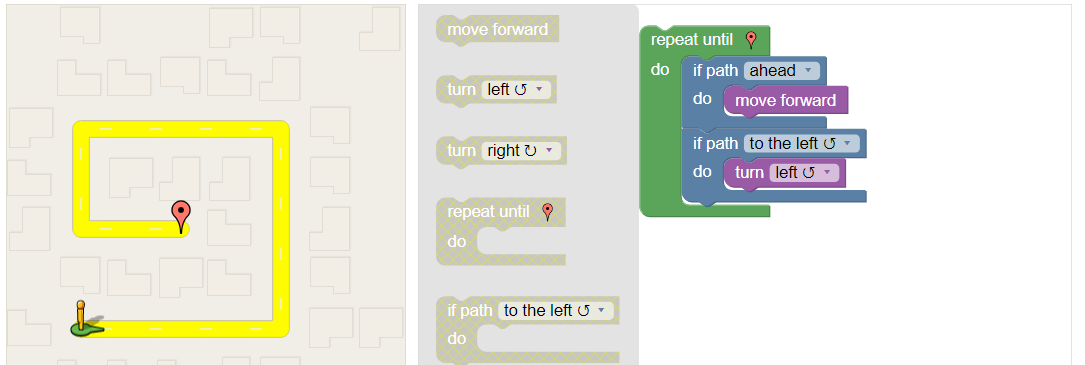
\includegraphics[width=1\textwidth]{pictures/blockly}
\caption{\emph{Blockly} ist eine grafische Programmiersprache von Google. Einzelne Elemente können miteinander kombiniert und verschaltet werden um kleine Programme zu entwickeln.}
\label{blockly}
\end{figure}

\subsection{Auszeichnungssprachen}
Eine weitere Möglichkeit zur komplexen Programmierung sind die sogenannten ver-einfachten Auszeichnungssprachen. Diese arbeiten mit Text der anhand einfacher Befehle formatiert und strukturiert wird. So kann anhand eines vorangehenden Symbols Text als Überschrift definiert werden. Insbesondere \emph{Markdown} verwendet Sonderzeichen um Textabschnitte zu formatieren und strukturieren (vgl. \cite{GettingS56:online}).

Auch \emph{YAML} nutzt Sonderzeichen, um Listen und größere Mengen von Daten zu beschreiben (vgl. \cite{TheOffic64:online}). \emph{BBCode} hingegen verwendet einfache Anweisungen die mit eckigen Klammern eingeleitet und abgeschlossen werden. Die Anweisung selbst wird in Form eines Buchstabens angegeben (vgl. \cite{BBCodeor24:online}).

\emph{HTML} ist die geläufigste Auszeichnungssprache. Diese wird zur Strukturierung von Websites benötigt. Dabei können verschiedene Bereiche definiert und deren Inhalte strukturiert werden. \emph{HTML} hat die Fähigkeit durch die Verwendung von Tags komplexe Inhalte, wie Texte, Bilder, Listen und Tabellen zu strukturieren und zu formatieren. Die Tags werden mit spitzen Klammern gekennzeichnet. Im Rahmen einer Studie wurde \emph{HTML} eingesetzt um Ambulante Assesment Protokolle zu erstellen, die sowohl vom Menschen lesbar als auch vom Computer ausführbar sind (vgl. \cite{Batalas2018}).

\begin{figure}[h]
\centering
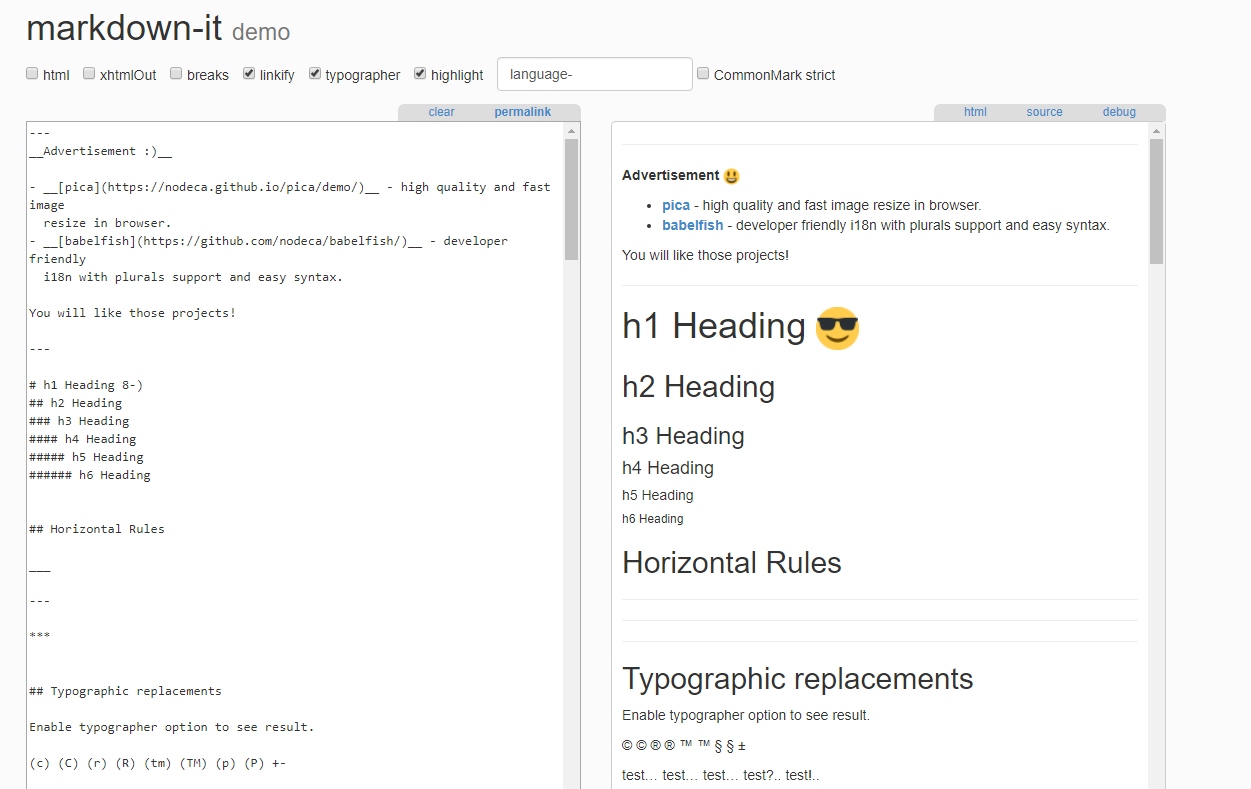
\includegraphics[width=1\textwidth]{pictures/markdown}
\caption{Die Auszeichnungssprache \emph{Markdown} verwendet verschiedene Sonderzeichen zur Strukturierung von Text}
\label{markdown}
\end{figure}



\subsection{Experience Sampling}
Psychotherapeuten und Psychologen haben die Möglichkeit anhand bestimmter Experience Sampling Software Fragebögen für mobile Geräte zu entwickeln (vgl. \cite{OSFSabri6:online}). Hierbei werden auch Lösungen angeboten, die  Auszeichnungssprachen verwenden. Die Software \emph{Experience Sampler} verwendet die Auszeichnungssprache \emph{JSON}, aufbauend auf \emph{YAML}, um Fragen, Anzeige- sowie Eingabeformate zu definieren (vgl. \cite{OSFSabri6:online}). \emph{MyExperience} verwendet einen ähnlichen Ansatz. Als Auszeichnungssprache zur Entwicklung der Fragebögen wird hier auf \emph{XML} zurückgegriffen (vgl. \cite{theMyExp48:online}).

Ein weiteres Projekt zur Erstellung von Experience Sampling ist \emph{Jeeves}. Fragebögen werden mit diesem Programm über eine grafische Programmiersprache definiert. Verwendet wird hauptsächlich die grafische Programmierung mit Blöcken. Über eine weitere Oberfläche werden die Eingabeformate der Antworten festgelegt. So ist es möglich Formate wie Likert Skala, Checkboxes, Radiobuttons, Ortsabfragen und weitere zu verwenden (vgl. \cite{Rough2017}).

Die Experience Sampling Software \emph{movisensXS} nutzt Diagramme zur Beschreibung des Ablaufs eines Fragebogens. Diese werden nach einem Puzzle-Prinzip angeordnet. Die Fragen selbst, sowie Formate der Antworten, werden separat angelegt und können später im Diagramm ausgewählt werden (vgl. \cite{movisens59:online}).

\begin{figure}[h]
\centering
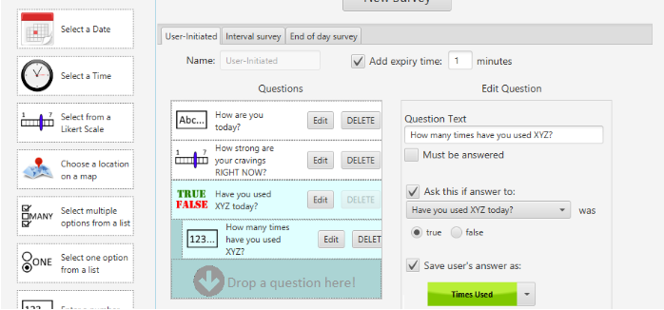
\includegraphics[width=1\textwidth]{pictures/jeeves}
\caption{Mit Hilfe von \emph{Jeeves} lassen sich Fragebögen für Experience Sampling erstellen. \cite{8e8f4fb047:online}}
\label{jeeves}
\end{figure}



\subsection{Fazit}

Zwar bieten Chatbot-Plattformen bereits einige Funktionen, allerdings fokussieren diese sich vornehmlich auf Marketing, Vertrieb und Support (vgl. \cite{Chatfuel3:online} \cite{Converse15:online} \cite{ManyChat78:online}). Dies kann die Umsetzung einer komplexen Therapie erschweren. Übliche Elemente, wie visuelle Analogskalen und Likert-Skalen, die häufig in der Psychologie Verwendung finden, können nur schwer oder gar nicht umgesetzt werden. Die Darstellungsformen der Konversationen verschiedener Chatbot-Plattformen haben unterschiedliche Vor- und Nachteile. Bäume und Diagramme bieten eine visuelle und leicht verständliche Übersicht eines Konversationsablaufs. Je größer und komplexer dieser Ablauf allerdings wird, umso unübersichtlicher wird eine Konversation. Bei großen Bäumen und Diagrammen werden in der Gesamtansicht die einzelnen Komponenten und Schriften zu klein und somit schwer Lesbar für das menschliche Auge. Ist die Funktion eines hinein- und herauszoomens implementiert, erschwert sich das verorten der Komponenten im Gesamtsystem (vgl. \cite{Hornbaek2003}). Blocksysteme bieten zusätzlich die visuelle Darstellung von Bedingungen, aber auch hier ist ein großer Konversationsablauf schnell unübersichtlich (vgl. \cite{Hornbaek2003}). Viele Elemente, die in Chatbot-Plattformen eingesetzt werden, könnten für einen Therapiemodellierungsansatz nützlich sein, da diese leicht nachvollziehbar und leicht in der Handhabung sind. Allerdings ist keine der bisherigen Chatbot-Plattformen derzeit geeignet, um eine komplexe Therapie umzusetzen ohne lange Einarbeitungszeit oder Einschränkungen in der Gestaltung. 

Auch eine Umsetzung mit den sogenannten grafischen Programmiersprachen wäre möglich um eigene Chatbots zu entwickeln. Überwiegend gibt es diese für spezielle Domänen wie Elektrotechnik. Das Baukastenprinzip ist hier besonders interessant, da es verschiedene Funktionen visuell darstellt und später in Code übersetzt. Die visuelle Darstellung ist leicht verständlich und schnell zu Erlernen. \emph{Blockly} bedient sich diesem Prinzip, um verschiedene Arten der Programmanweisungen verständlicher darzustellen. Allerdings erhält in dieser Form der Umsetzung ein komplexeres Programm oder System die zuvor genannten Probleme (vgl. \cite{Hornbaek2003}). Es gibt ebenfalls noch keine grafische Programmiersprache, die zur Umsetzung eines Therapiemodellierungsansatzes geeignet wäre. 

Für das Beschreiben einer Konversation wäre auch die Nutzung einer Auszeichnungssprache möglich. Das Schreiben eines Konversationsfluss wirkt hier sehr natürlich, da es dem Chatten nahe kommt. Aber auch hier kann man leicht die Übersicht verlieren, da Verzweigungen in Konversationen nicht entsprechend dargestellt werden können, wie es beispielsweise bei Diagrammen möglich ist. Auch liefern nicht alle Auszeichnungssprachen den Umfang von Funktionen um komplexe Therapien darzustellen. Auch die Syntax und Fehlersuche wird zeitaufwändig sofern das genutzte Programm zur Beschreibung keine oder eine rudimentäre Fehlerbehandlung mit sich bringt.  

Im Bereich des Experience Samplings werden bereits verschiedene Ansätze verwendet, die eine grafische Programmierung oder das Verwenden einer Auszeichnungssprache integrieren. Hier liegt der Fokus auf der Entwicklung von Fragebögen die zu verschiedenen Zeiten getriggert werden. Derzeit gibt es keine Experience Sampling Software die Therapien gezielt in Form von Konversationen umsetzt. Jedoch können Fragebögen ein wichtiges Stilmittel einer Therapie darstellen. 

Aufgrund der verschiedenen Vor- und Nachteile der vorgestellten Ansätze, wäre eine Kombination verschiedener Ansätze denkbar. 
